\section{Auswertung und Diskussion}
\label{sec:DiskussionAuswertung}
In den Abbildungen \ref{fig:eoxmitptv}, \ref{fig:eoymitptv} und \ref{fig:eoz} ist die Dosisverteilung in dem Schädel in der
Transversal-, Sagittal- und Frontalansicht zu sehen. In den Abbildungen ist zu erkennen, dass die $\SI{95}{\percent}$ Isodosenlinie das
rot eingezeichnete PTV in dem meisten Bereichen vollständig umschließt. Es ist lediglich in einem kleinen Teil des vorderen Bereichs des PTVs nicht
gelungen eine Dosis von $95\%$ zu erreichen. Das liegt daran, dass das PTV teilweise sehr nah an den Augen liegt und da die Augenlinsen durch die
MLCs geschützt werden sich dort keine relative Dosis von $95\%$ erreichen lässt. Außerdem ist zu erkennen, dass die maximale relative Dosis
$104,7\%$ außerhalb des PTVs liegt. Das kommt daher, da die Strahlenfelder das PTV aus lateraler Richtung bestrahlen und somit zunächst der Schädelknochen
durchquert werden muss, bevor das PTV erreicht wird. Aufgrund der hohen Dichte des Schädelknochens wird dort auch viel Dosis absorbiert.


Für eine bessere Beurteilung ist das Dosis-Volumen-Histogramm in der Abbildung \ref{fig:dvheinzel} gezeigt.

Da es sich bei dieser Erkrankung um eine gutartige Erkrankung handelt, ist es bei der Therapie wichtig das Gehirn möglichst gut zu schonen.
Bei dieser Therapie wird mit einer Gesamtdosis von $\SI{19.8}{\gray}$ bestrahlt und da der Organdosisgrenzwert für
das Gehirn bei $\SI{60}{\gray}$, wird der Grenzwert bei dieser Bestrahlung nicht überschritten \cite{QUANTEC}.

Die maximale relative Dosis in dem PTV liegt bei $\SI{103.7}{\percent}$ und überschreitet die maximale erlaubte relative Dosis von $\SI{107}{\percent}$
nicht \cite{ICRU}.
Die minimale Dosis, die im PTV deponiert wird, liegt bei $\SI{87.7}{\percent}$. Es konnte auch schon anhand der Dosisverteilung gesehen werden, dass
nicht im gesamten PTV eine relative Dosis von $95\%$ erreicht werden konnte. Allerdings ist auch zu erkennen, dass nur ein
sehr kleiner Teil des PTVs eine geringere Dosis als $95\%$ erhält.
In $\SI{99,3}{\percent}$ des
PTV Volumens wird $\SI{95}{\percent}$ der Dosis deponiert. Anhand des DVHs des gesamten Schädels (grüne Kurve) ist zu erkennen,
dass im gesamten Kopf nur eine relativ geringe Dosis deponiert wird. Nur etwa $6\%$ des Schädelvolumens erhält noch eine relative Dosis von
$50\%$.
Der Organdosisgrenzwert für die Linsen liegt bei $\SI{5}{\gray}$ \cite{grenz}. Die maximal Dosis der rechten Linse beträgt $\SI{3,74}{\gray}$ ($11\%$) und
der linken $\SI{2,18}{\gray}$ ($18,9\%$).
Daraus folgt, dass die Linsen ausreichend geschont werden konnten. Das ist auch in dem DVH zu erkennen,
weil die beiden Tiefendosiskurven relativ schnell abfallen.
Anhand der DVH Kurven der gesamten Augen ist zu erkennen, dass in den gesamten Augen relativ viel Dosis deponiert wird.
In etwa $64\%$ des rechten Auges und in etwa $51\%$ des linken Auges werden noch $50\%$ des Dosis deponiert. Das kommt daher, da
das PTV teilweise sehr nah an den Augen liegt. Deshalb ist es nicht möglich die Augen besser zu schützen. \\

Insgesamt lässt sich sagen, dass durch diesen Bestrahlungsplan mit zwei opponierenden Feldern die gewünschte Dosisverteilung im Zielvolumen
gut erreicht wird. Außerdem konnten mit diesem Bestrahlungsplan die Organdosisgrenzwerte eingehalten werden.

\begin{figure}[h]
	\centering
	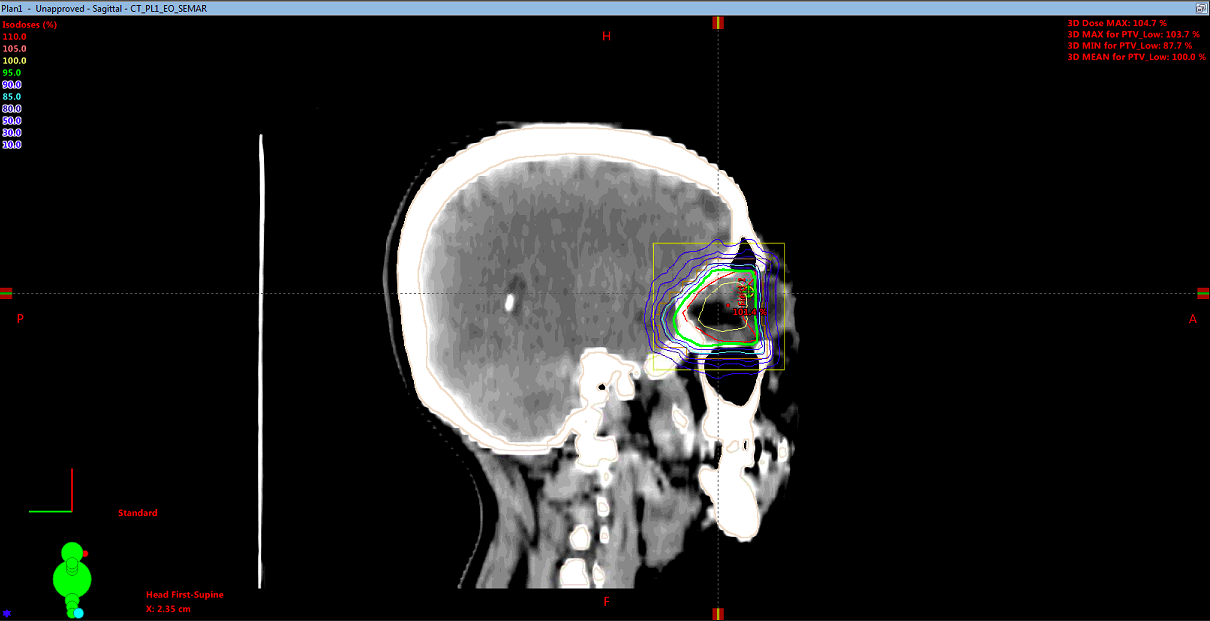
\includegraphics[width=\linewidth]{Bilder/EO_X_mitPTV}
	\caption{Darstellung der Dosisverteilung in der Sagittalansicht des Schädels.}
	\label{fig:eoxmitptv}
\end{figure}

\begin{figure}[h]
	\centering
	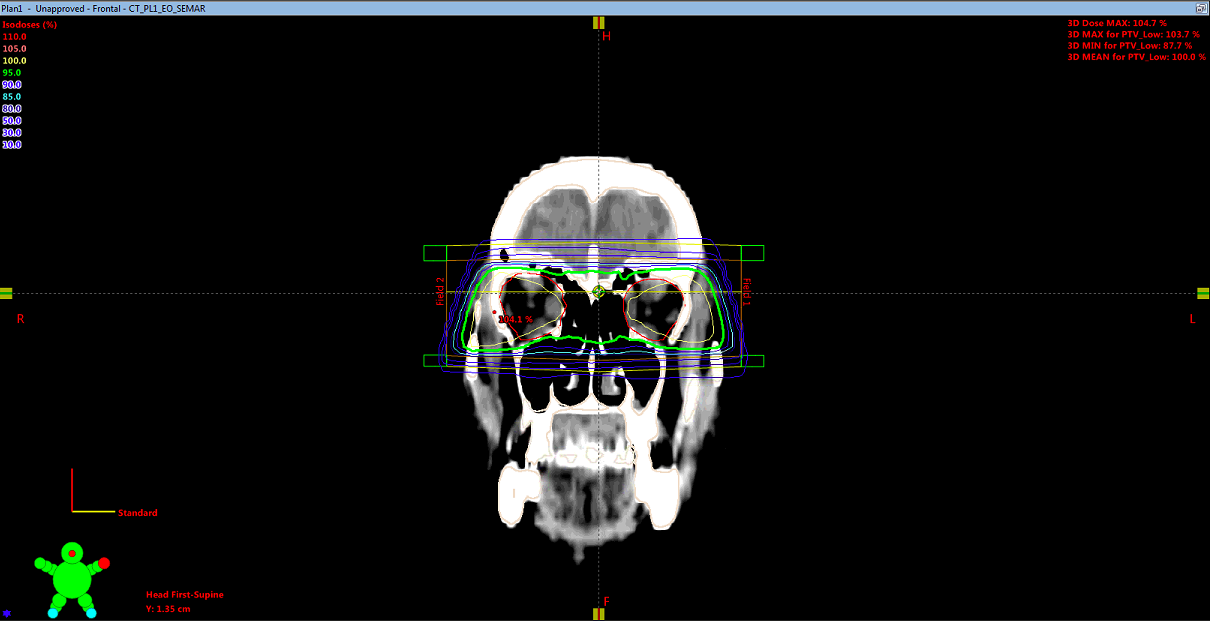
\includegraphics[width=\linewidth]{Bilder/EO_Y_mitPTV}
	\caption{Darstellung der Dosisverteilung in der Frontalansicht des Schädels.}
	\label{fig:eoymitptv}
\end{figure}

\begin{figure}[h]
	\centering
	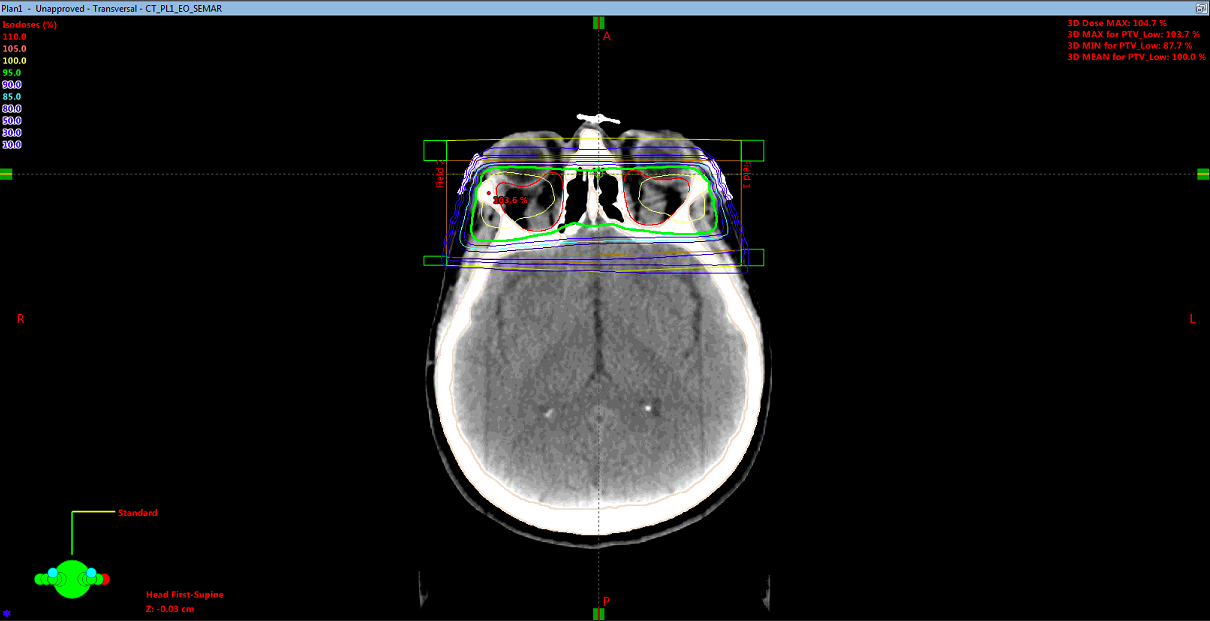
\includegraphics[width=\linewidth]{Bilder/EO_Z}
	\caption{Darstellung der Dosisverteilung in der Transversalansicht des Schädels.}
	\label{fig:eoz}
\end{figure}

\begin{figure}[h]
	\centering
	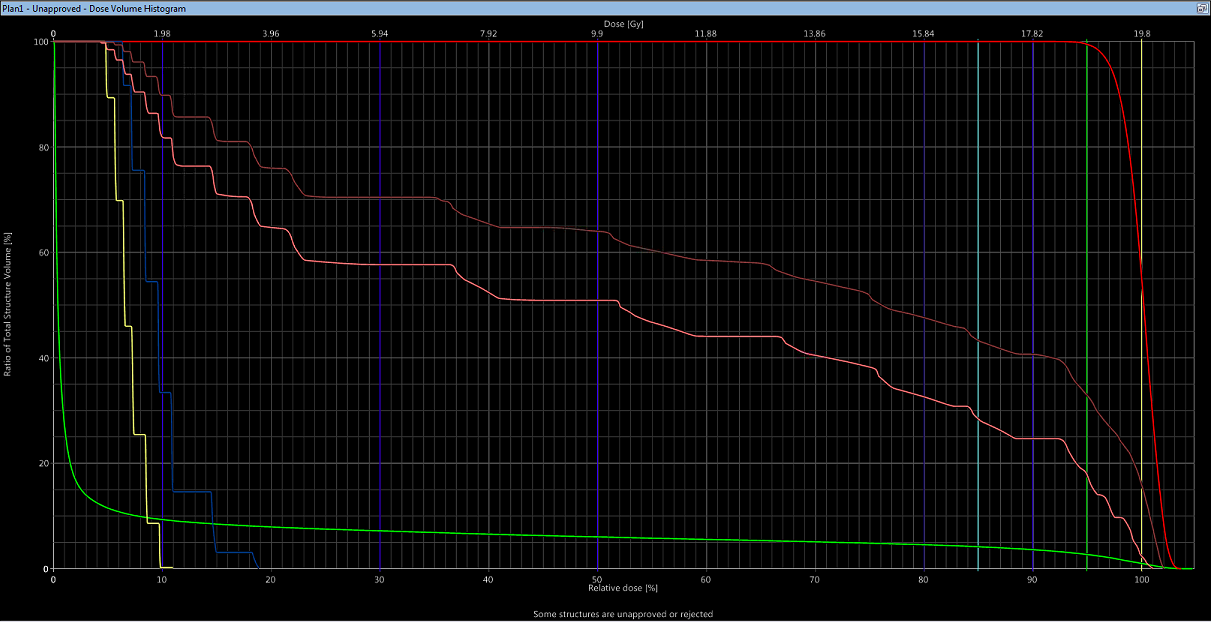
\includegraphics[width=\linewidth]{Bilder/DVH_Einzel}
	\caption{Zu sehen ist das DVH des Schädels. In roter Farbe dargestellt ist das PTV und in grüner Farbe ist der Schädel. Außerdem sind noch die einzelnen Isodosenlinien eingezeichnet und die einzelnen Kurven zu den Risikoorgane wie z.B. von den Linsen (gelb, dunkelblau) und Augen (pink,braun).}
	\label{fig:dvheinzel}
\end{figure}
